\chapter{Grundriss Prototyp} \label{ch:grRiss}
	In den bisherigen Prototypen wurde die Migration auf das Modulsystem von Java behandelt. Jedoch ist das Problem des dynamischen Ladens und Auswechselns von Plugins während der Laufzeit, nicht thematisiert worden. Dieser Prototyp erarbeitet mithilfe der neu eingeführten Konzepte des Modulsystems, einen möglichen Grundriss für die dynamische Umsetzung eines Plugin-Systems. Hierfür werden die Module, die Modulschichten, sowie der Java \textit{Service-Lader}, eingesetzt. Da die Plugin-Module keine oder wenig Logik in sich tragen, werden sie in diesem Kapitel als Plugin-Fassade bezeichnet.

\section{Anforderungen} 
	Zurzeit können die Plugins in die laufende Applikation integriert werden. Dazu wird die eingebaute Funktion des Klassen-Laders genutzt. Der Klassenlader kann neue Plugin-Code in das System integriert, jedoch können die geladenen Plugins im Nachhinein nicht mehr entladen werden. Dementsprechend soll erforscht werden, ob mithilfe des Modulsystems, eine Lösung für das bestehende Problem gefunden werden kann. Für die Lösung soll ein Grundriss Prototyp entstehen, welcher das dynamische Laden und Entladen der Plugins skizziert. Der Prototyp soll keine lauffähige Logik von \textsc{Renew} oder \textsc{Mulan} umsetzen, sondern das Laden und Entladen von Java-Code darstellen.

\section{Spezifikation} 
	Für die Umsetzung wird der aktuelle Zustand von \textsc{Renew} begutachtet, und zuvor erarbeitete, aber nicht integrierte Lösungsansätze, zusammengefasst. Die nachfolgende Anfertigung des konzeptionellen Grundrisses erstellt eine Modulschicht per Plugin und verknüpft die Plugins miteinander über die Schichtendelegation, sowie die \textit{Service-Lader} Instanz. Das Ergebnis stellt eine Fassade dar, die nachfolgend als ein Grundriss implementiert und ausgewertet wird.

\section{Entwurf} \label{sec:entwurf}
	Die grundlegende Idee der Modulschichten und des \textit{Service-Laders}, wurde im Kapitel \ref{sec:module_layers} und \ref{sec:servLoad} diskutiert. Mithilfe der Module, Modulschichten und des \textit{Service-Laders} wird in diesem Abschnitt ein Grundriss des möglichen Einsatzes im Plugin-Management vorgestellt. \bigbreak

	Das zentrale Problem der zurzeit betriebenen Umsetzung, ist das monolithische Verhalten der Plugins, die sich den gleichen Klassenraum teilen, direkte Zugriffe durchführen und während der Laufzeit, nicht voneinander getrennt werden können. Denn die \textsc{Renew}-Plugins sind an den Plugin-Klassenlader gebunden und dürfen laut der Java Plattform, diesen nicht mehr verlassen. \newline
	Um die Plugins aus der Applikation endgültig zu entfernen, müssen die Plugins auf separate Klassenlader aufgeteilt und betrieben werden. Durch den Einsatz von mehreren Klassenlader, kann die Referenz auf ein bestimmtes Klassenlader Objekt, welches ein Plugin in sich trägt, gelöscht, oder neu belegt werden. Somit ist das ehemalige Klassenlader-Objekt nicht mehr erreichbar und wird von dem \textit{Garbage Collector} aus dem Speicher entfernt.\bigbreak 

	Wie bereits in den Grundlagen Kapitel \ref{cha:Grundlagen} behandelt, sind die zur Verfügung gestellten Klassenlader hierarchisch aufgebaut, arbeiten nach dem \textit{Parent First} Delegationsprinzip und können die Anfrage nur an einen übergeordneten Klassenlader delegieren. Dementsprechend fehlt dem Klassenlader-System die Integration der verzweigten Delegation sowie die organisierte Kommunikation zwischen einer variablen Anzahl an Klassenlader, die für das Plugin-System eine große Rolle spielen.\newline
	Mit der Integration der Module und Modulschichten in die Java Plattform, sollen die angesprochenen Probleme adressiert und gelöst werden. Aus diesem Grund kümmert sich das Modulsystem von Java um die Authentizität, sowie Integrität des Modulinhalts und führt zusätzlich das Konzept der Modulschichten ein, welches das Verwalten der System-Modulbausteine übernimmt und den genauen Aufenthaltsort jedes Moduls, sowie seiner zuständigen Verwaltungsinstanz, überblickt. Da die \textsc{Renew}-Plugins als Module umgesetzt worden sind, genießen sie die Eigenschaften der Module, sowie die Unterstützung des Modulsystems.\newline
	Die Verwaltung des Plugin-Inhalts und dessen Abhängigkeiten, werden über die expliziten Schnittstellen angegeben und über eine Konfiguration, die einen Teil der Modulschicht darstellt, validiert. Die Konfiguration erstellt einen Plugin-Abhängigkeitsgraphen, der aus einer gegebenen Verzeichnismenge einem ausgewählten Wurzel-Plugin und einer optionalen Anzahl von untergeordneten Konfigurationen, Plugin-Beziehungen herstellt. Die Konfiguration validiert und stellt sicher, dass alle benötigten Abhängigkeiten gefunden und aufgelöst werden, keine Zyklen durch das Hinzufügen neuer Plugins, sowie Bibliothek entstehen und jedes Plugin, sowie jede Bibliothek, eindeutig jeder Suchanfrage zugeordnet werden kann. Somit überblickt die Konfiguration der Modulkonstellation und den Zustand ihrer Schicht, sowie der darunterliegenden Modulschichten. Dies hat zur Folge, dass Plugins und Drittanbieter-Bibliotheken nur einmal in der Schicht-Konfiguration auftreten können, und verhindern somit das Überladen von bestehender Funktionalität.\newline
	Die elastische Konfigurationseinstellung und die globale Konsistenz der modularen Applikation, ermöglichen eine verzweigte Delegation der Suchanfrage an bekannte Modulschichten und dessen Plugin-Module, die zuvor validiert und in die Applikation eingebettet worden sind. Somit kennt die Applikation alle Plugins, sowie die dazugehörigen Bibliotheken und kann die Suchanfrage an die entsprechende Schicht weiterleiten, ohne ein Sicherheitsrisiko einzugehen.\newline
	Die neu eingeführte verzweigte Delegation spielt eine große Rolle für das Plugin Konzept, denn die Plugins erweitern und werden von anderen zahlreichen Plugins erweitert. Die dynamische Zusammensetzung der Plugins kann ohne Struktur und umfassende Sicherheitsmechanismen in einem großen System, nicht mängelfrei bestehen. Dementsprechend muss das erweiternde Plugin von unerwarteten äußeren Einflüssen geschützt werden, und vor dem Einbinden in die Applikation, eine valide Strukturintegration nachweisen. Die genannten Anforderungen werden bestens von den Modulen und den Modulschichten abgedeckt, die mit der zusätzlichen verzweigten Delegation, neue Möglichkeiten der Java Plattform  und somit auch \textsc{Renew} bieten.\bigbreak

	Im Folgenden wird ein Prototyp vorgestellt, der ein Plugin System simuliert, welches aus Modulen, sowie  Modulschichten besteht und als ein Grundriss für die mögliche Umsetzung der nächsten \textsc{Renew} Version die dienen könnte. \bigbreak
			
	\begin{figure}[t]
		   \centering
		   \captionsetup{justification=centering}
		   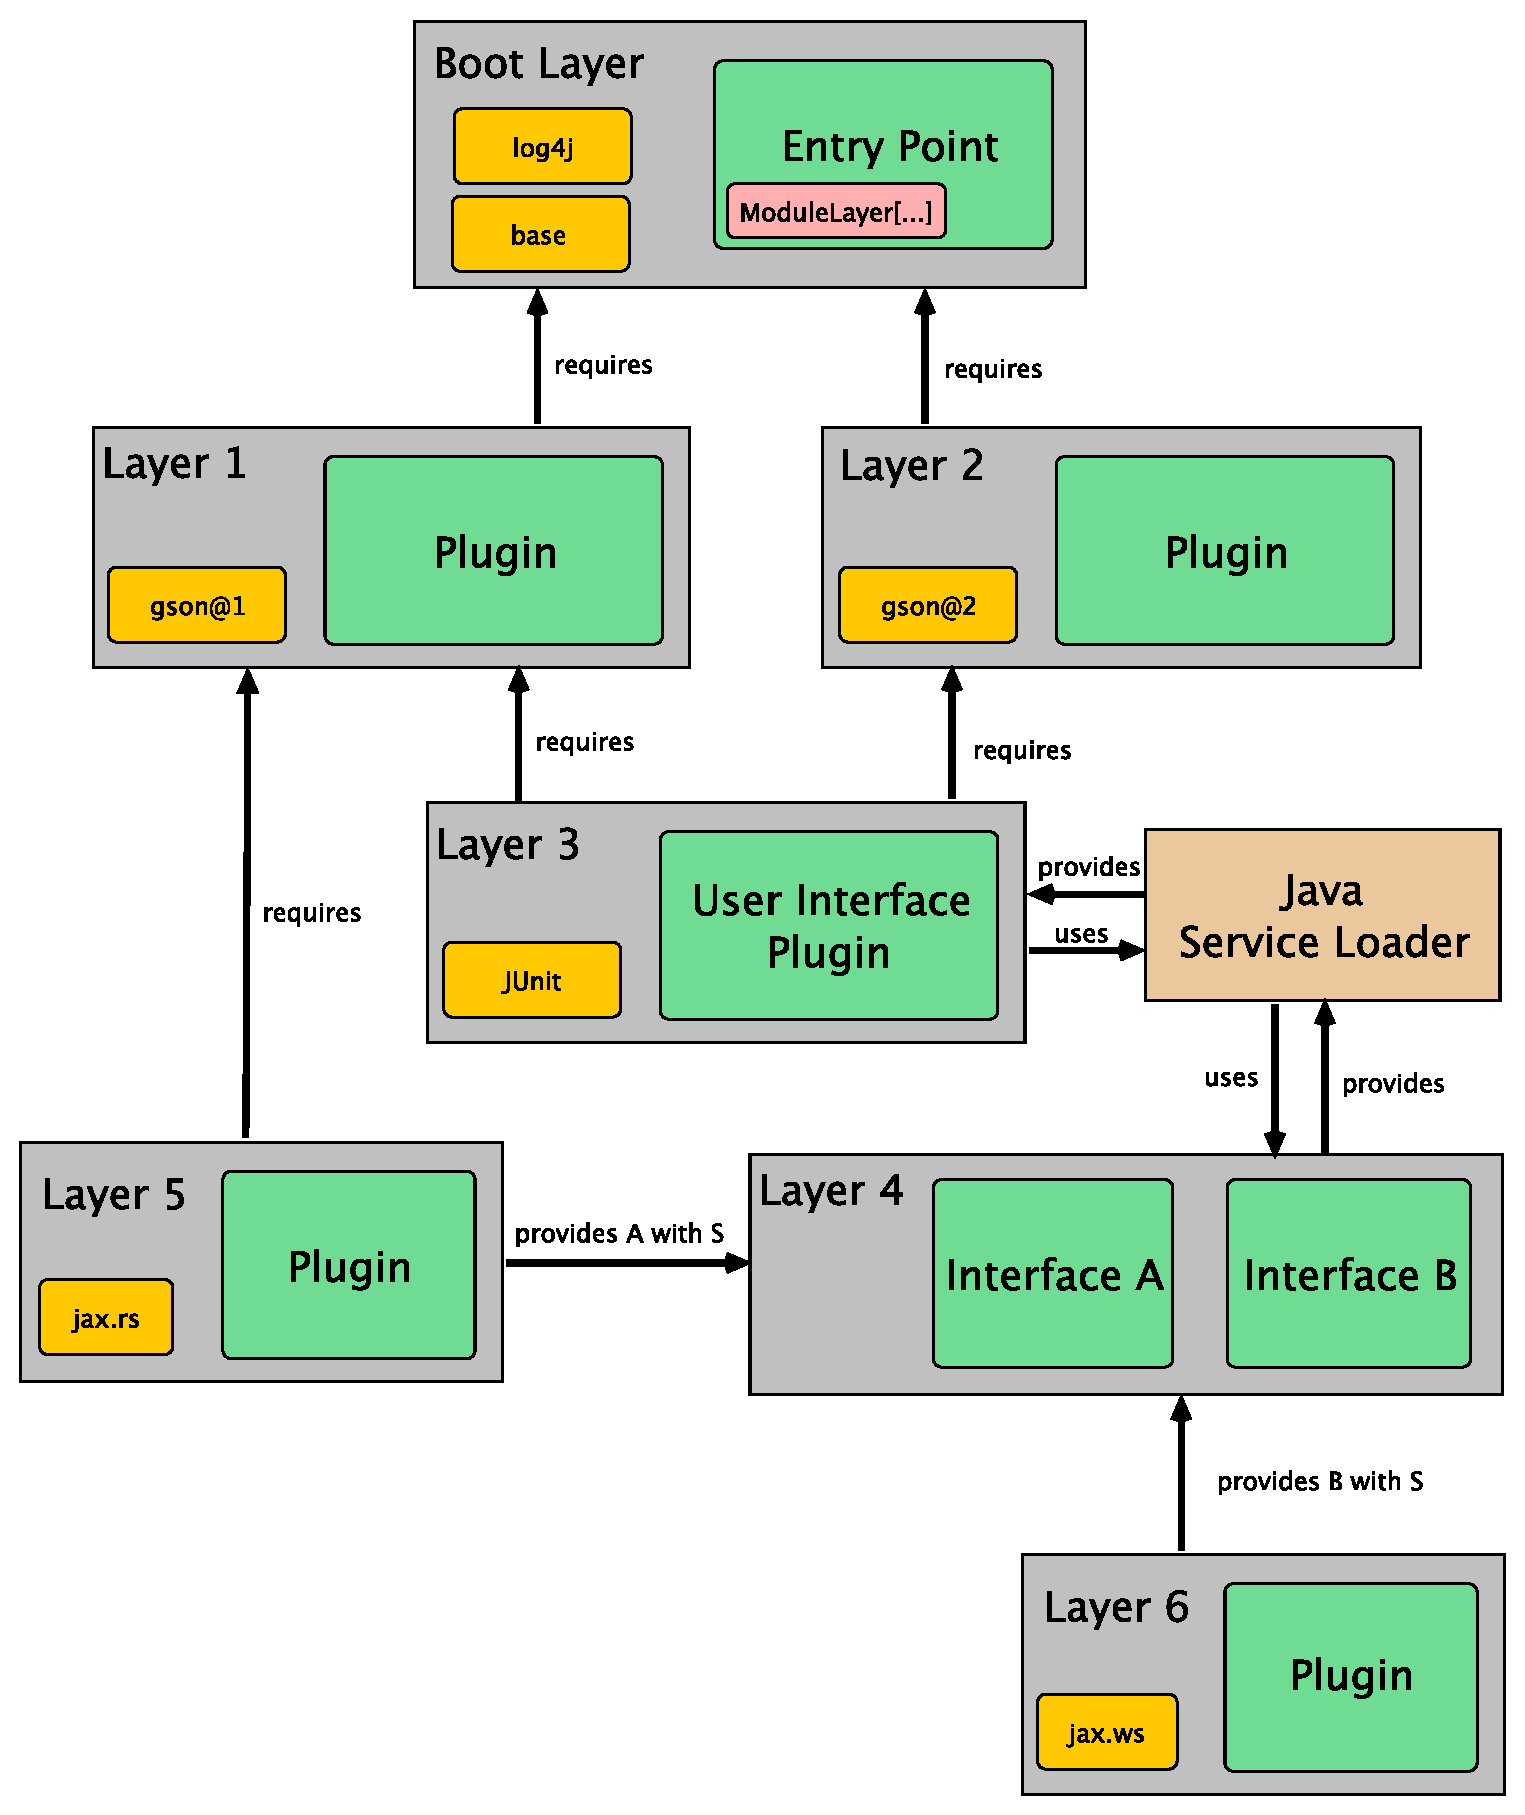
\includegraphics[width=0.8\textwidth]{material/images/ModulLayerDepsDraw.pdf}
		   \caption{Grundriss einer möglichen Plugin-Architektur auf Basis der Modulschichten}
		   \label{fig:ModSchichtKonzept}
	\end{figure}
\newpage	
	Die Abbildung \ref{fig:ModSchichtKonzept} visualisiert den Grundriss. Ganz oben in der Schichtenhierarchie, befindet sich die \textit{Boot-Schicht}. Diese enthält die von Java zur Verfügung gestellten Module, sowie den Einstiegspunkt der Applikation. Der Einstiegspunkt der Applikation erstellt und verwaltet die Plugins über die zur Laufzeit erstellten Modulschichten. Die darunterliegenden Schichten \textit{Layer 1} und \textit{Layer 2}, stellen zwei unterschiedliche Plugin Funktionalitäten dar, die in unterschiedlicher Version dieselbe Bibliothek \textit{gson} nutzen und die Möglichkeit des parallelen Betriebs illustrieren. Die Modulschicht \textit{Layer 3} baut auf der \textit{Layer 2} und \textit{Layer 3} Modulschicht auf und benötigt dessen Funktionalität für die eignen Implementation. Zum Beispiel könnte es die Funktion des \textit{UI}-Plugins darstellen, die die \textit{Util}, sowie \textit{WindowManagment} Plugins aus der \textit{Layer 2}, sowie \textit{Layer 3} Modulschicht anfordert. Dementsprechend kann ein Plugin mithilfe der Modulschichten zwei oder mehr übergeordnete Schichten referenzieren und konfliktfrei auf ihre Funktionalität zugreifen.\newline
	Da das \textit{UI}-Plugin nicht auf allen \textsc{Renew}-Plugins aufbaut, sondern diese lediglich koordiniert, muss die parallel entstehende Logik aus der Schicht \textit{Layer 5}, für das \textit{UI}-Plugin zugänglich gemacht werden. Dies wird mithilfe des Java \textit{Service-Laders} umgesetzt, der für ein gegebenes Schnittstellenmodul und einer Schicht, alle zugänglichen Implementationen erfasst und als ein Dienst für die Ausführung dem \textit{UI}-Plugin anbietet. Dafür deklariert das \textit{UI}-Plugin aus der Schicht \textit{Layer 3} eine Abhängigkeit und eine Dienstnutzung auf die Schnittstellenmodule aus der Schicht \textit{Layer 4}. Die Schicht \textit{Layer 4} enthält zwei Schnittstellenmodule, die nur für das UI-Plugin Dienste anbieten und werden in dieser Umsetzung praktischerweise, in einer Schicht, zusammengefasst. Dennoch könne die Schnittstellenmodule auf separate Schichten aufgeteilt und verwaltet werden. \newline 
	Für den Aufruf der Dienstsuche, wird auf die \textit{ModuleLayer} Liste aus dem \textit{Entry-Point}-Plugin zugegriffen, und über alle Elternschichten, nach Diensten gesucht. Wenn ein Solcher gefunden wurde, instanziiert der \textit{Service-Lader} die Dienstklassen und bietet sie den \textit{UI}-Plugin, für die Nutzung an. Somit ist das Laden und Entladen neuer Plugins in die Applikation möglich, und kann während der Laufzeit durchgeführt werden.  

\section{Umsetzung}\label{sec:umsetzung}
	Für die Erstellung einer Schicht, wird eine \textit{createLayer(...)} Methode implementiert, die für eine neue Konfiguration bestehend aus der übergeordneten Modulschichtliste, eine Modulverzeichnis, und  einem Wurzelmodulnamen.  Dafür wird zuerst aus jeder Modulschicht die Konfiguration ausgelesen und in der folgenden Auflösung des Modulgraphen verwendet. Demnach wird der Graph aus Modulen der übergeordneten Konfigurationen, einschließlich aller Module aus dem Modulwurzelverzeichnis, erstellt und von einer neuen Konfiguration umhüllt.\bigbreak
	\begin{figure}[h!]
		   \centering
		   \captionsetup{justification=centering}
		   \includegraphics[width=\textwidth]{material/images/umsetzung/configs.pdf}
		   \caption{Die \textit{createLayer} Methode}
		   \label{fig:layerCreation}
	\end{figure}
	Dadurch ist sichergestellt, dass alle Abhängigkeiten erfüllt sind und die Software betriebsfähig ist. Dennoch besteht die neu erstellte Konfiguration nur aus Metainformation über die Modulkonstellation, und wird folglich von der Modulschicht verarbeitet. Die neue Modulschicht nimmt die erstellte Konfiguration, samt der zugrundeliegenden Modulschichtenliste auf, um die Modul- und Klassensuche, an die entsprechende Schicht, zu delegieren. Für die Unterstützung des alten Klassenlader-Konzepts und dem nicht modularisierten Teil der Applikation, muss zusätzlich ein übergeordneter Klassenlader angegeben werden, der in diesem Fall, immer auf den \textit{System-Klassenlader} verweist. Somit werden die expliziten, sowie automatischen Module, von dem Modulsystem betreut und genießt den Vorteil der direkten Delegation, sowie der Suchdelegation, an mehrere übergeordnete Modulschichten. Im Gegensatz dazu, arbeitet der nicht modularisierte Teil der Applikation, weiterhin parallel auf dem alten Klassenlader-Konzept, mit nur einer übergeordneten Elterndelegation und dem \textit{parent first} Ansatz. Das vorgestellt Verfahren wird in der Abbildung \ref{fig:layerCreation} abgebildet.\bigbreak
	\begin{figure}[h!]
		   \centering
		   \captionsetup{justification=centering}
		   \includegraphics[width=0.6\textwidth]{material/images/umsetzung/left.pdf}
		   \caption{Erstellung der Schichtenhierarchie}
		   \label{fig:createlayer}
	\end{figure}
	Nachdem die Modulschichten erstellt werden können, wird von der \textit{Starter}-Plugin-Fassade die Schichtenhierarchie aufgebaut und verknüpft. Dafür werden zuerst die Schichten erzeugt, die an die \textit{Boot-Schicht} angebunden sind, wie zum Beispiel die Schicht mit der Plugin-Fassade-\textit{left}. Die errichteten Schichten dienen nun selbes, als übergeordnete Modulschichten für Plugin-Fassaden, die deren Logik erweitern möchten. \newline
	Zum Beispiel benötigt die \textit{UI}-Plugin-Fassade die Logik aus der Schicht \textit{left}, \textit{right} und \textit{services}, um ihre Funktion erfüllen zu können. Dementsprechend wird eine Modulschicht für die \textit{UI}-Plugins-Fassade erstellt, die auf den benötigten Modulschichten aufbaut und diese als übergeordnet, deklariert. Die dargestellte Vorgehensweise wird in der Abbildung \ref{fig:createlayer} visualisiert.\newpage
	\begin{figure}[h!]
		   \centering
		   \captionsetup{justification=centering}
		   \includegraphics[width=0.8\textwidth]{material/images/umsetzung/main.pdf}
		    \caption{Aufruf der Applikation und des Dienstes}
		   \label{fig:figgi}
	\end{figure}
	Um die Applikation zu starten, wird die \textit{main} Methode der \textit{UI}-Plugin-Fassade aufgerufen, indem über die passende Modulschicht nach der Plugin-Fassade gesucht, und dessen \textit{main} Methode mittels \textit{Reflexion}, aufgerufen wird. Somit ähnelt der Applikationsaufbau der \textsc{Renew} Umsetzung. Denn es muss zuerst eine Delegationshierarchie errichtet (s. \ref{fig:classLoadDuv}) werden, die anschließend verwaltet und betrieben wird. \newline
	Zum Schluss, ruft die \textit{UI}-Plugin-Fassade den \textit{Service-Lader} auf, um auf die dynamisch eingebunden Dienste zuzugreifen. Dafür wird über die \textit{Service-Lader} Instanz, eine Suche aus einer gegebenen Modulschicht und einer Dienstschnittstelle durchgeführt, um alle möglichen Implementationen zur Verfügung zu stellen. Die Dienst-Implementation kann anschließend die angeforderte Funktionalität umsetzen. In der Abbildung \ref{fig:figgi} wird der Name des Dienstes auf die Konsole ausgegeben. \bigbreak 

\section{Evaluation}
	Der Grundriss-Prototyp hat sein Ziel erreicht und beschreibt mithilfe des Modulsystems ein Vorgehen, für das Erstellen einer dynamischen Applikation. Jedoch ist beim Erarbeiten des Grundrisses, unerwartetes Verhalten festgestellt worden. Die Modulschicht sollte für die Applikation eine Modulabhängigkeitsgraphen erstellen, der für die Ausführung nur notwendige Module enthält und nicht benötigte Module außen vor lässt. Dieses Verhalten wird von dem Modulsystem nur zum Teil verfolgt, denn die automatischen Module tragen in sich keine Modulbeschriftungen, und werden aus diesem Grund von der Java Plattform an alle Module in der entsprechenden Schicht gekoppelt. Somit ist jedes Modul in einer Schicht mit jedem automatischen Modul verbunden, auch wenn diese miteinander nicht interagieren. Daraus folgt ein unnötiges Laden aller automatischen Module aus der gegebenen Ordnerstruktur, und macht das Verwalten von nicht modularisierten Drittanbieter Bibliotheken aus einer zentralen Stelle, problematisch. Da \textsc{Renew} alle Drittanbieter Bibliotheken aus einem Verzeichnis steuert, muss für die saubere Schichtenbildung jedes Plugin mit den genutzten Drittanbieter-Bibliothek, separat organisiert werden.\newline
	Ein weiteres unvorhergesehenes Problem entsteht durch die elastische Delegation der Klassen- und Modulsuche, die auf mehrere Modulschichten verteilt werden kann und trotzdem die Konsistenz der Applikation garantiert.
	Durch die variable Anzahl an Modulschichten, können parallel gleichnamige Bibliotheken betrieben werden, ohne die Konsistenz der Applikation infrage zu stellen. Dies geschieht zum Beispiel durch den Aufbau einer zusätzlichen Schicht, die auf Schichten mit gleichnamigen oder ähnlichen Bibliotheken aufsetzt. Jedoch ist die Konsistenz nicht in allen Fällen der genannten Struktur gegeben. \newline
	Die Existenz eines Moduls in mehreren Schichten erzeugt keine Probleme, da die Schicht festgelegt und nicht verändert werden kann, und die Suche nach den Modulen in einer strikten Ordnung, durchgeführt wird. Dennoch können Module ihre Funktionalität transitiv an die darüberliegenden Module und Schichten anknüpfen, und somit eine Inkonsistenz erzeugen. Denn die Suche kann nun nicht entscheiden, welche für das Modul zur Verfügung gestellten Implementation ausgewählt werden soll. \newline
